\chapter{Les mécanismes d'exécution d'un programme}
\lecture{2}{Mardi 23 Septembre 13:10}{Mécanismes d'exécution}
\section{Opcodes et languages machines}
\begin{enumerate}
\item Dans un ordi
\begin{itemize}
  \item Instruction = suite de 0 et 1
  \item Programme = suite d'instructions
  \item programme = longue suite de 0 et 1 (transformée en mnémonics pour la lecture)
  \item Programme stocké en MR centrale
\end{itemize}
\item Language humain = \textbf{Mnémonics}
\item Programmer en assembleur = mapping = Mnémonics -> Opcodes 
\end{enumerate}

\section{Mapping mnémoniques et registres (AR1)}
\begin{enumerate}
\item Mnemonic et Opcode
\begin{itemize}
  \item add = 000
  \item sub = 001
  \item load = 010
  \item store = 011
\end{itemize}
\item Registre et binary code
\begin{itemize}
  \item A = 00
  \item B = 01
  \item C = 10
  \item D = 11
\end{itemize}
\section{Instruction add avec registres}
\begin{itemize}
  \item 0 = mode
  \item 1,2,3 = opcode
  \item 4,5 = source 1 
  \item 6,7 = source 2
  \item 8,9 = destination
  \item 10->15 = 00000000
\end{itemize}
\begin{itemize}
  \item Si le premier bit est 0 -> manipulations registres
  \item Si 1 -> Valeurs immédiates sont utilisées
  \item Les 6 derniers bits complètent l'écriture sur 2 octets, remplir l'espace disponible(padding)
  \item Exemple: add C, D, A = 00001011 00000000
  \item 0 premier bit de mode -> Manipulations registres
\end{itemize}
\section{Instruction add avec valeurs immédiates}
\begin{itemize}
\item 0 = mode
\item 1,2,3 = opcode
\item 4,5 = source
\item 6,7 = destination
\item 8->15 = 8 bit immediate value
\item = instruction set
\end{itemize}
\begin{itemize}
  \item Exemple: add C, 8, A = 10001000 00001000
  \item 1 premier bit de mode -> Valeurs immédiates
  \item 8 -> sur 8 bits = 00001000
\end{itemize}
\item Remarques importantes
\begin{itemize}
  \item Augmenter le nombre de bits utilisés pour coder une opération ou un register permet d'augmenter le nombre d'opérations et de registres disponibles. 
  \item 2 bits -> 4 possibilités
  \item 3 bits -> 8 possibilités
  \item 4 bits -> 16 possibilités
  \item 2 exposant nombre de bits - les bits utilisés pour les opérations des registres (destination, mode ect...)
\end{itemize}
  \item Les opérations ainsi disponibles forment \textbf{l'instruction set}
\end{enumerate}

\section{Instruction load avec type immédiat}
\begin{enumerate}
\item Type immédiat (immediate-type load)
\item Sur 16 bits:
\begin{itemize}
  \item 0 = mode -> va être à 1 du à opération immédiate
  \item 1,2,3 = opcode
  \item 4,5 = source -> 00 -> vu qu'opération immédiate pas de registre padding "00"
  \item 6,7 = destination
  \item 8->15 = 8 bit immediate value
\end{itemize}
\item Exemple: load \#12, A = 10100000 00001100 -> Charger le contenu de A avec la valeur pointé par l'adresse 12
\item 010 = load \# un autre opcode existe pour load sans \#
\end{enumerate}

\section{Instruction load avec registre}
\begin{enumerate}
\item Type avec registre sur 16 bits:
\begin{itemize}
  \item 0 = mode -> 0 car opération avec registre
  \item 1,2,3 = opcode
  \item 4,5 = source
  \item 6,7 = 00
  \item 8,9 = destination
  \item 10->15 = 8 bit immediate value
\end{itemize}
\end{enumerate}

\section{Instruction load avec base + offset}
\begin{enumerate}
\item Type avec base + offset sur 16 bits:
\begin{itemize}
  \item 0 = mode
  \item 1,2,3 = opcode
  \item 4,5 = base
  \item 6,7 = destination 
  \item 8->15 = 8 bit immediate value
\end{itemize}
\item Exemple: load \#12, A = 10100000 00001100
\item store C, \#14 = 10111000 00001110
\end{enumerate}

\section{L'assembleur}
\begin{enumerate}
\item Avant:
\begin{itemize}
  \item Programme réalisé en logique cablée
  \item Charger/modifier/adapter un programme -> modification physique des circuits de l'ordinateur
  \item Le résultat apparait sous forme binaire également
  \item un clavier ou un écran aurait demandé un ordinateur à eux-seuls pour fonctionner
  \item Pas d'intégration de fonctions logiques
  \item Pas de RAM -> relais = bascules à mémoire
\end{itemize}
\item Maintenant:
\begin{itemize}
  \item Développements technologiques
  \item Intégration tech -> plus de puissance
  \item Création de mémoires contenant des programmes
  \item Traitement de texte en programmes (compilateur)
  \item exemples: Bandes perforées
\end{itemize}

\section{Compilateur}
\item Fonctionnement du compilateur, il va lister les instructions de cette manière:
\begin{itemize}
\item load
\item store
\item add
\item ...
\item il simplifie la tâche
\item Besoin de connaître les ressources dispo:
  \begin{itemize}
    \item Nombre de registres
    \item instructions supportées
    \item Adressage mémoire (où)
    \item Comment ces registres vont fonctionner
  \end{itemize}
\end{itemize}
\item Ce modèle se nomme \textbf{programming model}
\centering
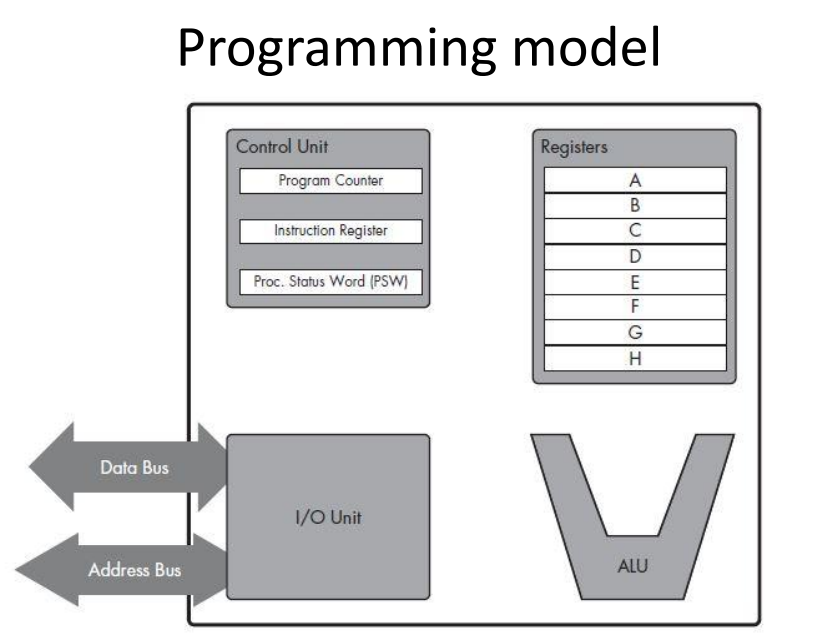
\includegraphics[scale=0.3]{programming-model}
\vfill
l'ALU et l'I/O unit vont travailler, le bus d'adressage n'est utilisé que par le microprocesseur pour donner les adresses.
\end{enumerate}

\section{program counter}
\begin{enumerate}
\item le CPU va lire les instructions à suivre dans le programme. Pas modifiable à priori sauf dans certains cas. 
\item Pointe vers la prochaine adresse à lire ou à écrire.
\item Met l'info sur le bus d'adresse.
\item Incrémentage automatique par le microprocesseur. JMP instructions peuvent modifier celui-ci.
\end{enumerate}
\begin{itemize}
  \item opcode
  \item source
  \item destination
  \item mode
\end{itemize}

\section{instruction register}
\begin{enumerate}
  \item Lorsque l'instruction est lue, elle sera mise dans l'instruction register pour être décoder et exécutée. 
  \item Flux de données et flux d'instructions. 
  \item Permet au microprocesseur de savoir quelle instruction exécuter. Les registres servent comme destination pour les résultats des instructions, ils peuvent aussi servir comme sources.
\end{enumerate}

\section{Proc Status Word (PSW)}
\begin{enumerate}
  \item Sert pour les instructions JMP, garde le statut d'une condition (JPMZ, JMPN, JMPE)
  \item Sert à définir l'overflow, le négatif...
\end{enumerate}

\section{Stack Register}
\begin{enumerate}
\item Si saut -> utilisation du PC en y stockant la valeur du PC depuis lequel on jump dans la stack
Jump vers l'élément = call 
\item Puis retour dans le cours du programme grâce à la valeur dans la stack au dessus de la pile et l'enlever de cette pile vers le PC = return 
\end{enumerate}

\section{Fetch-Decode-Execute}
\begin{enumerate}
  \item \textbf{Fetch} est une action du CPU qui \textbf{lit une donnée en MR}
  \item A l'adresse \textbf{PC} (program counter)
  \item L'envoie à \textbf{l'IR (instruction register)} 
  \item \textbf{Decode opcode/source/destination/mode}
  \item \textbf{Execute l'instruction quand il a besoin dans un cas complexe}
  \item Le PC est incrémenté (ou modifié par l'instruction exécutée)
  \item Quand l'exécution est terminée, le cycle reprend
\end{enumerate}

\subsection{exemple}
\begin{enumerate}
\item PC = 500 -> IR = load \#12, A ; Envoi du contenu de la cellule 12 dans le PC et le bus d'adresse
\item PC = 502 -> IR = load \#13, B
\item PC = 504 -> IR = add A,B,C ; Plus rien dans le bus d'adresse (pas de valeur immédiate) recherche seulement dans le microprocesseur
\item PC = 506 -> IR = store C, \#14 ; Envoi de la cellule mémoire 14 dans le bus d'adresse (mémoire RAM ou I/O car besoin d'écriture) pour stocker la valeur contenue dans C  
\end{enumerate}

\section{recap dans AR1}
\begin{enumerate}
\item Les cellules mémoires ont une taille de 1 octet (8 bits)
\item Les instructions ont un format sur 2 octets
\item Pour les instructions, il faut charger 2 octets pour avoir une instructions
\item Il faut incrémenter le PC de 2 à chaque instruction
\end{enumerate}
